\documentclass{standalone}
\usepackage{tikz}
\usetikzlibrary{patterns, positioning}
\usepackage[sfdefault]{ClearSans} %% option 'sfdefault' activates Clear Sans as the default text font
\usepackage[T1]{fontenc}

\begin{document}
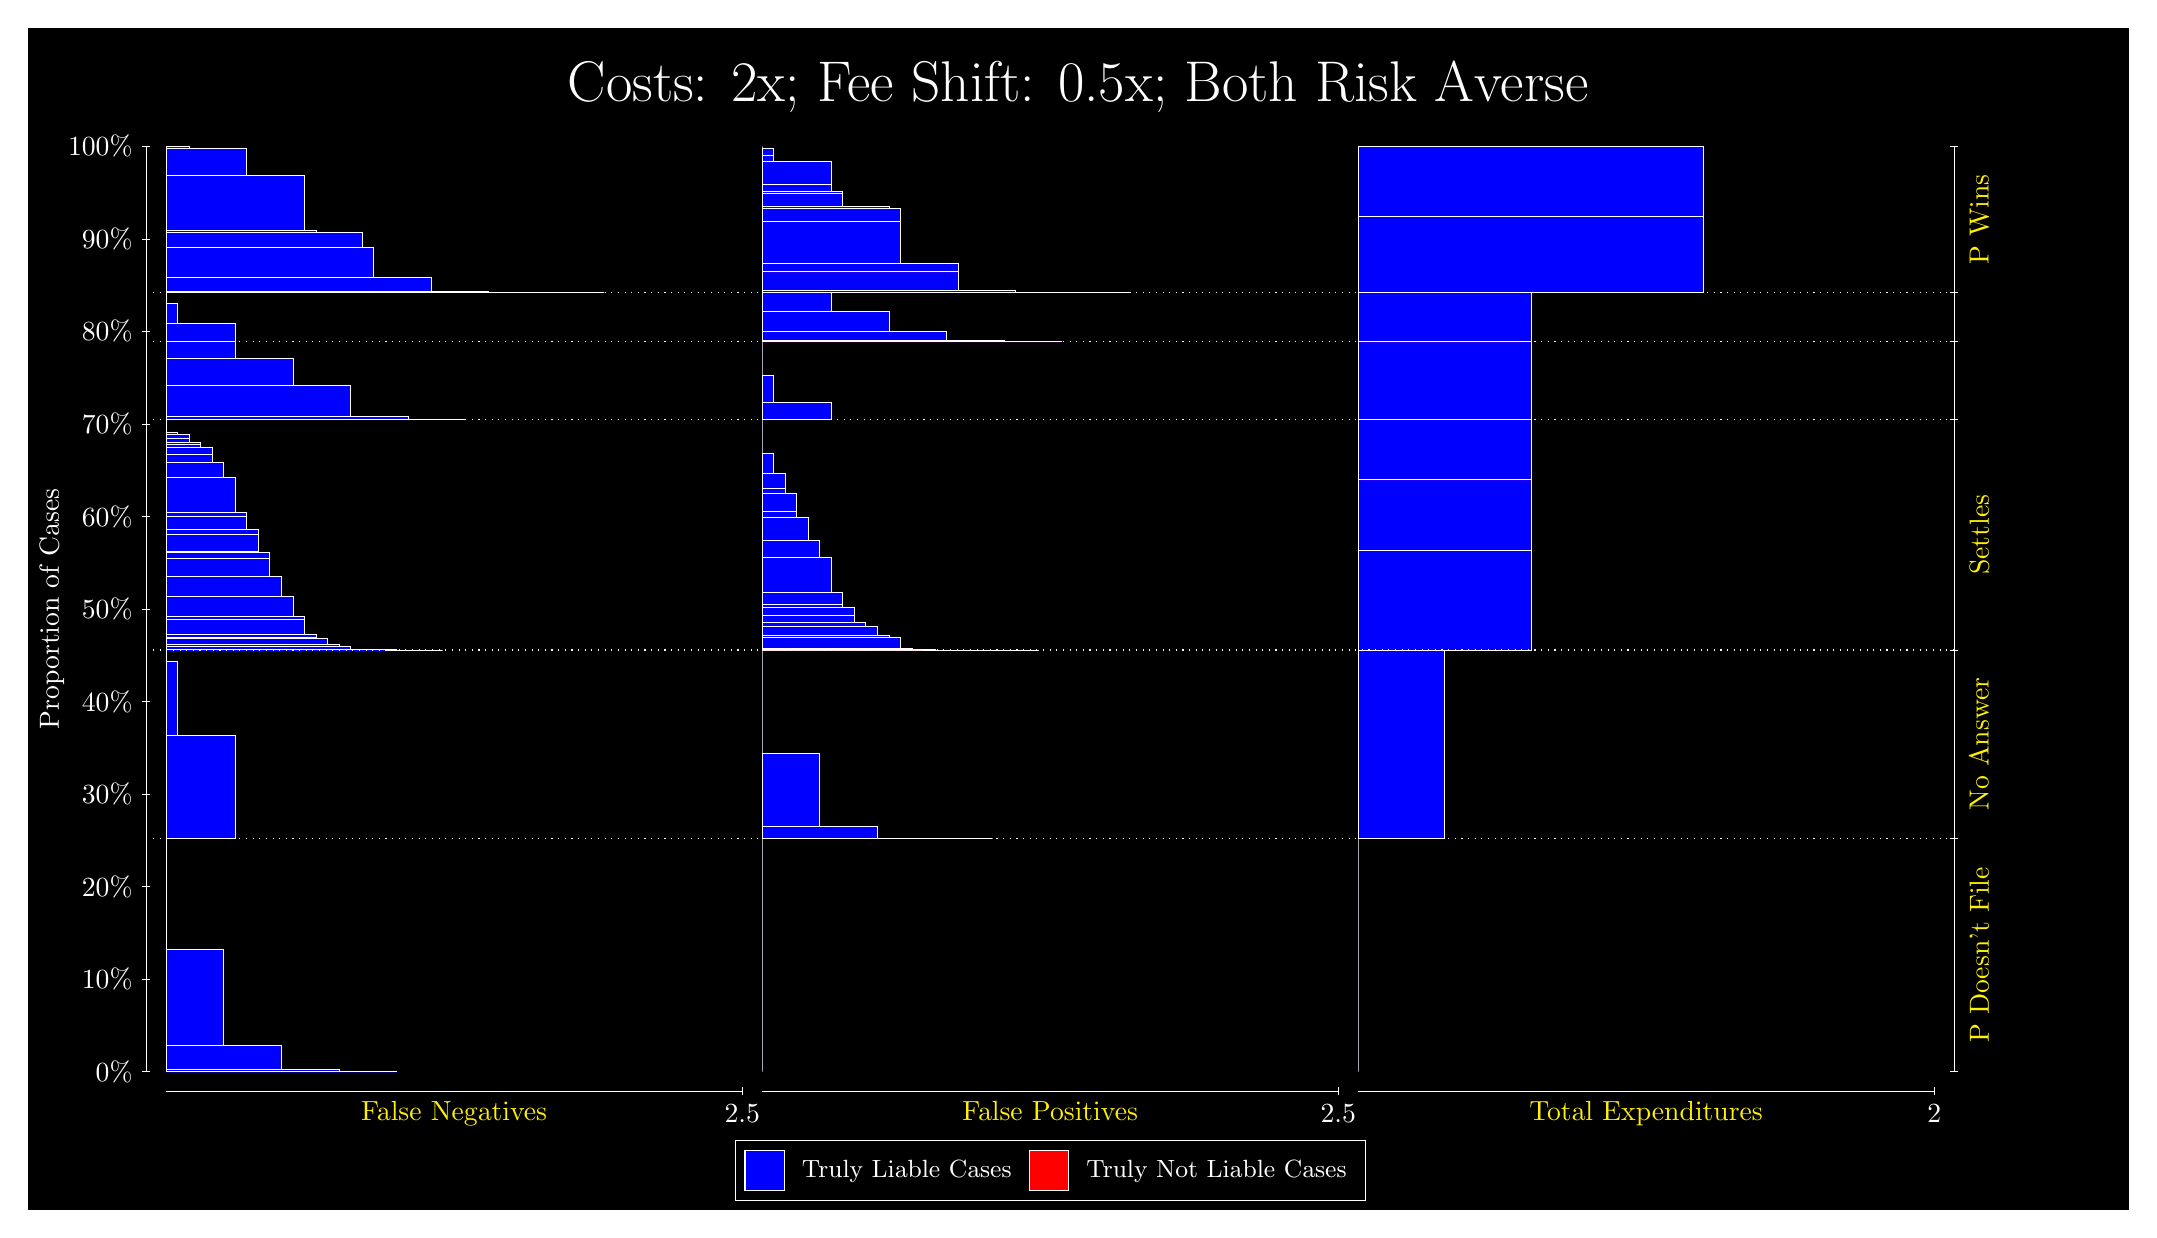
\begin{tikzpicture}
\draw[fill=black] (0,0) rectangle (26.667,15);
\draw[text=white] (0,13.5) rectangle (26.667,15) node[midway] {\huge Costs: 2x; Fee Shift: 0.5x; Both Risk Averse};
\draw[white, very thin] (1.5,1.75) -- (1.5,13.5);
\node[rotate=90, text=white, anchor=center] at (0.3, 7.625) {Proportion of Cases};
\draw[white, very thin] (1.45,1.75) -- (1.55,1.75);
\node[text=white, anchor=east] at (1.45, 1.75) {0\%};
\draw[white, very thin] (1.45,2.925) -- (1.55,2.925);
\node[text=white, anchor=east] at (1.45, 2.925) {10\%};
\draw[white, very thin] (1.45,4.1) -- (1.55,4.1);
\node[text=white, anchor=east] at (1.45, 4.1) {20\%};
\draw[white, very thin] (1.45,5.275) -- (1.55,5.275);
\node[text=white, anchor=east] at (1.45, 5.275) {30\%};
\draw[white, very thin] (1.45,6.45) -- (1.55,6.45);
\node[text=white, anchor=east] at (1.45, 6.45) {40\%};
\draw[white, very thin] (1.45,7.625) -- (1.55,7.625);
\node[text=white, anchor=east] at (1.45, 7.625) {50\%};
\draw[white, very thin] (1.45,8.8) -- (1.55,8.8);
\node[text=white, anchor=east] at (1.45, 8.8) {60\%};
\draw[white, very thin] (1.45,9.975) -- (1.55,9.975);
\node[text=white, anchor=east] at (1.45, 9.975) {70\%};
\draw[white, very thin] (1.45,11.15) -- (1.55,11.15);
\node[text=white, anchor=east] at (1.45, 11.15) {80\%};
\draw[white, very thin] (1.45,12.325) -- (1.55,12.325);
\node[text=white, anchor=east] at (1.45, 12.325) {90\%};
\draw[white, very thin] (1.45,13.5) -- (1.55,13.5);
\node[text=white, anchor=east] at (1.45, 13.5) {100\%};

\draw[white, very thin] (24.457,1.75) -- (24.457,13.5);
\draw[white, very thin] (24.407,1.75) -- (24.507,1.75);
\node[anchor=west] at (24.407, 1.75) {};
\draw[white, very thin] (24.407,4.7119) -- (24.507,4.7119);
\node[anchor=west] at (24.407, 4.7119) {};
\draw[white, very thin] (24.407,7.104) -- (24.507,7.104);
\node[anchor=west] at (24.407, 7.104) {};
\draw[white, very thin] (24.407,10.031) -- (24.507,10.031);
\node[anchor=west] at (24.407, 10.031) {};
\draw[white, very thin] (24.407,11.019) -- (24.507,11.019);
\node[anchor=west] at (24.407, 11.019) {};
\draw[white, very thin] (24.407,11.645) -- (24.507,11.645);
\node[anchor=west] at (24.407, 11.645) {};
\draw[white, very thin] (24.407,13.5) -- (24.507,13.5);
\node[anchor=west] at (24.407, 13.5) {};

\draw[white, very thin, fill=blue] (1.75,1.75) rectangle (4.6775,1.7502);
\draw[white, very thin, fill=blue] (1.75,1.7502) rectangle (3.9457,1.7726);
\draw[white, very thin, fill=blue] (1.75,1.7726) rectangle (3.2138,2.086);
\draw[white, very thin, fill=blue] (1.75,2.086) rectangle (2.4819,3.2977);
\draw[white, very thin, fill=red] (1.75,3.2977) rectangle (1.75,3.2977);
\draw[white, very thin, fill=blue] (1.75,3.2977) rectangle (1.75,4.7119);
\draw[white, very thin, fill=blue] (1.75,4.7119) rectangle (2.6283,6.0257);
\draw[white, very thin, fill=blue] (1.75,6.0257) rectangle (1.8964,6.9573);
\draw[white, very thin, fill=red] (1.75,6.9573) rectangle (1.75,6.9573);
\draw[white, very thin, fill=blue] (1.75,6.9573) rectangle (1.75,7.104);
\draw[white, very thin, fill=blue] (1.75,7.104) rectangle (5.2631,7.104);
\draw[white, very thin, fill=blue] (1.75,7.104) rectangle (4.9703,7.104);
\draw[white, very thin, fill=blue] (1.75,7.104) rectangle (4.6775,7.107);
\draw[white, very thin, fill=blue] (1.75,7.107) rectangle (4.5312,7.1092);
\draw[white, very thin, fill=blue] (1.75,7.1092) rectangle (4.3848,7.1093);
\draw[white, very thin, fill=blue] (1.75,7.1093) rectangle (4.3848,7.1122);
\draw[white, very thin, fill=blue] (1.75,7.1122) rectangle (4.2384,7.1164);
\draw[white, very thin, fill=blue] (1.75,7.1164) rectangle (4.092,7.1446);
\draw[white, very thin, fill=blue] (1.75,7.1446) rectangle (3.9457,7.1801);
\draw[white, very thin, fill=blue] (1.75,7.1801) rectangle (3.7993,7.255);
\draw[white, very thin, fill=blue] (1.75,7.255) rectangle (3.6529,7.2607);
\draw[white, very thin, fill=blue] (1.75,7.2607) rectangle (3.6529,7.3024);
\draw[white, very thin, fill=blue] (1.75,7.3024) rectangle (3.5065,7.4892);
\draw[white, very thin, fill=blue] (1.75,7.4892) rectangle (3.5065,7.5308);
\draw[white, very thin, fill=blue] (1.75,7.5308) rectangle (3.3602,7.7862);
\draw[white, very thin, fill=blue] (1.75,7.7862) rectangle (3.2138,8.0404);
\draw[white, very thin, fill=blue] (1.75,8.0404) rectangle (3.0674,8.2648);
\draw[white, very thin, fill=blue] (1.75,8.2648) rectangle (3.0674,8.3448);
\draw[white, very thin, fill=blue] (1.75,8.3448) rectangle (2.921,8.36);
\draw[white, very thin, fill=blue] (1.75,8.36) rectangle (2.921,8.5686);
\draw[white, very thin, fill=blue] (1.75,8.5686) rectangle (2.921,8.6336);
\draw[white, very thin, fill=blue] (1.75,8.6336) rectangle (2.7746,8.803);
\draw[white, very thin, fill=blue] (1.75,8.803) rectangle (2.7746,8.8563);
\draw[white, very thin, fill=blue] (1.75,8.8563) rectangle (2.6283,9.2939);
\draw[white, very thin, fill=blue] (1.75,9.2939) rectangle (2.4819,9.4884);
\draw[white, very thin, fill=blue] (1.75,9.4884) rectangle (2.3355,9.585);
\draw[white, very thin, fill=blue] (1.75,9.585) rectangle (2.3355,9.6748);
\draw[white, very thin, fill=blue] (1.75,9.6748) rectangle (2.1891,9.6769);
\draw[white, very thin, fill=blue] (1.75,9.6769) rectangle (2.1891,9.7163);
\draw[white, very thin, fill=blue] (1.75,9.7163) rectangle (2.1891,9.7358);
\draw[white, very thin, fill=blue] (1.75,9.7358) rectangle (2.0428,9.7889);
\draw[white, very thin, fill=blue] (1.75,9.7889) rectangle (2.0428,9.8388);
\draw[white, very thin, fill=blue] (1.75,9.8388) rectangle (1.8964,9.8705);
\draw[white, very thin, fill=red] (1.75,9.8705) rectangle (1.75,9.8705);
\draw[white, very thin, fill=blue] (1.75,9.8705) rectangle (1.75,10.031);
\draw[white, very thin, fill=blue] (1.75,10.031) rectangle (5.5558,10.032);
\draw[white, very thin, fill=blue] (1.75,10.032) rectangle (4.8239,10.069);
\draw[white, very thin, fill=blue] (1.75,10.069) rectangle (4.092,10.459);
\draw[white, very thin, fill=blue] (1.75,10.459) rectangle (3.3602,10.803);
\draw[white, very thin, fill=blue] (1.75,10.803) rectangle (2.6283,11.019);
\draw[white, very thin, fill=red] (1.75,11.019) rectangle (1.75,11.019);
\draw[white, very thin, fill=blue] (1.75,11.019) rectangle (2.6283,11.256);
\draw[white, very thin, fill=blue] (1.75,11.256) rectangle (1.8964,11.512);
\draw[white, very thin, fill=red] (1.75,11.512) rectangle (1.75,11.512);
\draw[white, very thin, fill=blue] (1.75,11.512) rectangle (1.75,11.645);
\draw[white, very thin, fill=blue] (1.75,11.645) rectangle (7.3123,11.645);
\draw[white, very thin, fill=blue] (1.75,11.645) rectangle (6.5805,11.646);
\draw[white, very thin, fill=blue] (1.75,11.646) rectangle (5.8486,11.665);
\draw[white, very thin, fill=blue] (1.75,11.665) rectangle (5.7022,11.665);
\draw[white, very thin, fill=blue] (1.75,11.665) rectangle (5.1167,11.833);
\draw[white, very thin, fill=blue] (1.75,11.833) rectangle (4.9703,11.839);
\draw[white, very thin, fill=blue] (1.75,11.839) rectangle (4.3848,12.218);
\draw[white, very thin, fill=blue] (1.75,12.218) rectangle (4.2384,12.41);
\draw[white, very thin, fill=blue] (1.75,12.41) rectangle (3.6529,12.438);
\draw[white, very thin, fill=blue] (1.75,12.438) rectangle (3.5065,13.126);
\draw[white, very thin, fill=blue] (1.75,13.126) rectangle (2.921,13.126);
\draw[white, very thin, fill=blue] (1.75,13.126) rectangle (2.7746,13.47);
\draw[white, very thin, fill=blue] (1.75,13.47) rectangle (2.0428,13.5);
\draw[white, very thin, fill=red] (1.75,13.5) rectangle (1.75,13.5);
\draw[white, very thin, fill=blue] (1.75,13.5) rectangle (1.75,13.5);
\draw[white, very thin, fill=red] (9.3189,1.75) rectangle (9.3189,1.75);
\draw[white, very thin, fill=blue] (9.3189,1.75) rectangle (9.3189,4.7119);
\draw[white, very thin, fill=red] (9.3189,4.7119) rectangle (12.246,4.7119);
\draw[white, very thin, fill=blue] (9.3189,4.7119) rectangle (12.246,4.7119);
\draw[white, very thin, fill=blue] (9.3189,4.7119) rectangle (11.515,4.7126);
\draw[white, very thin, fill=blue] (9.3189,4.7126) rectangle (10.783,4.8586);
\draw[white, very thin, fill=blue] (9.3189,4.8586) rectangle (10.051,5.7901);
\draw[white, very thin, fill=blue] (9.3189,5.7901) rectangle (9.3189,7.104);
\draw[white, very thin, fill=red] (9.3189,7.104) rectangle (12.832,7.104);
\draw[white, very thin, fill=blue] (9.3189,7.104) rectangle (12.832,7.104);
\draw[white, very thin, fill=red] (9.3189,7.104) rectangle (12.539,7.104);
\draw[white, very thin, fill=blue] (9.3189,7.104) rectangle (12.539,7.104);
\draw[white, very thin, fill=red] (9.3189,7.104) rectangle (12.246,7.104);
\draw[white, very thin, fill=blue] (9.3189,7.104) rectangle (12.246,7.104);
\draw[white, very thin, fill=blue] (9.3189,7.104) rectangle (12.1,7.1046);
\draw[white, very thin, fill=red] (9.3189,7.1046) rectangle (11.954,7.1046);
\draw[white, very thin, fill=blue] (9.3189,7.1046) rectangle (11.954,7.1046);
\draw[white, very thin, fill=blue] (9.3189,7.1046) rectangle (11.807,7.1053);
\draw[white, very thin, fill=red] (9.3189,7.1053) rectangle (11.661,7.1053);
\draw[white, very thin, fill=blue] (9.3189,7.1053) rectangle (11.661,7.1055);
\draw[white, very thin, fill=blue] (9.3189,7.1055) rectangle (11.515,7.1089);
\draw[white, very thin, fill=red] (9.3189,7.1089) rectangle (11.368,7.1089);
\draw[white, very thin, fill=blue] (9.3189,7.1089) rectangle (11.368,7.1144);
\draw[white, very thin, fill=blue] (9.3189,7.1144) rectangle (11.222,7.1198);
\draw[white, very thin, fill=blue] (9.3189,7.1198) rectangle (11.075,7.1284);
\draw[white, very thin, fill=red] (9.3189,7.1284) rectangle (11.075,7.1284);
\draw[white, very thin, fill=blue] (9.3189,7.1284) rectangle (11.075,7.2649);
\draw[white, very thin, fill=blue] (9.3189,7.2649) rectangle (10.929,7.2966);
\draw[white, very thin, fill=red] (9.3189,7.2966) rectangle (10.783,7.2966);
\draw[white, very thin, fill=blue] (9.3189,7.2966) rectangle (10.783,7.3996);
\draw[white, very thin, fill=blue] (9.3189,7.3996) rectangle (10.636,7.4606);
\draw[white, very thin, fill=red] (9.3189,7.4606) rectangle (10.49,7.4606);
\draw[white, very thin, fill=blue] (9.3189,7.4606) rectangle (10.49,7.5504);
\draw[white, very thin, fill=blue] (9.3189,7.5504) rectangle (10.49,7.647);
\draw[white, very thin, fill=blue] (9.3189,7.647) rectangle (10.344,7.6811);
\draw[white, very thin, fill=blue] (9.3189,7.6811) rectangle (10.344,7.8414);
\draw[white, very thin, fill=blue] (9.3189,7.8414) rectangle (10.197,8.2791);
\draw[white, very thin, fill=blue] (9.3189,8.2791) rectangle (10.051,8.5018);
\draw[white, very thin, fill=blue] (9.3189,8.5018) rectangle (9.9044,8.7905);
\draw[white, very thin, fill=blue] (9.3189,8.7905) rectangle (9.758,8.8706);
\draw[white, very thin, fill=blue] (9.3189,8.8706) rectangle (9.758,9.095);
\draw[white, very thin, fill=blue] (9.3189,9.095) rectangle (9.6116,9.1561);
\draw[white, very thin, fill=blue] (9.3189,9.1561) rectangle (9.6116,9.3492);
\draw[white, very thin, fill=blue] (9.3189,9.3492) rectangle (9.4652,9.6046);
\draw[white, very thin, fill=blue] (9.3189,9.6046) rectangle (9.3189,10.031);
\draw[white, very thin, fill=red] (9.3189,10.031) rectangle (10.197,10.031);
\draw[white, very thin, fill=blue] (9.3189,10.031) rectangle (10.197,10.248);
\draw[white, very thin, fill=blue] (9.3189,10.248) rectangle (9.4652,10.592);
\draw[white, very thin, fill=blue] (9.3189,10.592) rectangle (9.3189,11.019);
\draw[white, very thin, fill=red] (9.3189,11.019) rectangle (13.125,11.019);
\draw[white, very thin, fill=blue] (9.3189,11.019) rectangle (13.125,11.019);
\draw[white, very thin, fill=blue] (9.3189,11.019) rectangle (12.393,11.033);
\draw[white, very thin, fill=blue] (9.3189,11.033) rectangle (11.661,11.153);
\draw[white, very thin, fill=blue] (9.3189,11.153) rectangle (10.929,11.409);
\draw[white, very thin, fill=blue] (9.3189,11.409) rectangle (10.197,11.645);
\draw[white, very thin, fill=red] (9.3189,11.645) rectangle (14.003,11.645);
\draw[white, very thin, fill=blue] (9.3189,11.645) rectangle (14.003,11.645);
\draw[white, very thin, fill=red] (9.3189,11.645) rectangle (13.271,11.645);
\draw[white, very thin, fill=blue] (9.3189,11.645) rectangle (13.271,11.646);
\draw[white, very thin, fill=red] (9.3189,11.646) rectangle (12.539,11.646);
\draw[white, very thin, fill=blue] (9.3189,11.646) rectangle (12.539,11.675);
\draw[white, very thin, fill=blue] (9.3189,11.675) rectangle (11.807,11.909);
\draw[white, very thin, fill=red] (9.3189,11.909) rectangle (11.807,11.909);
\draw[white, very thin, fill=blue] (9.3189,11.909) rectangle (11.807,12.019);
\draw[white, very thin, fill=red] (9.3189,12.019) rectangle (11.661,12.019);
\draw[white, very thin, fill=blue] (9.3189,12.019) rectangle (11.661,12.019);
\draw[white, very thin, fill=blue] (9.3189,12.019) rectangle (11.075,12.552);
\draw[white, very thin, fill=blue] (9.3189,12.552) rectangle (11.075,12.707);
\draw[white, very thin, fill=red] (9.3189,12.707) rectangle (10.929,12.707);
\draw[white, very thin, fill=blue] (9.3189,12.707) rectangle (10.929,12.736);
\draw[white, very thin, fill=blue] (9.3189,12.736) rectangle (10.344,12.905);
\draw[white, very thin, fill=blue] (9.3189,12.905) rectangle (10.344,12.927);
\draw[white, very thin, fill=blue] (9.3189,12.927) rectangle (10.197,13.013);
\draw[white, very thin, fill=red] (9.3189,13.013) rectangle (10.197,13.013);
\draw[white, very thin, fill=blue] (9.3189,13.013) rectangle (10.197,13.306);
\draw[white, very thin, fill=blue] (9.3189,13.306) rectangle (9.6116,13.311);
\draw[white, very thin, fill=blue] (9.3189,13.311) rectangle (9.6116,13.313);
\draw[white, very thin, fill=blue] (9.3189,13.313) rectangle (9.4652,13.386);
\draw[white, very thin, fill=blue] (9.3189,13.386) rectangle (9.4652,13.481);
\draw[white, very thin, fill=blue] (9.3189,13.481) rectangle (9.3189,13.5);
\draw[white, very thin, fill=red] (16.888,1.75) rectangle (16.888,1.75);
\draw[white, very thin, fill=blue] (16.888,1.75) rectangle (16.888,4.7119);
\draw[white, very thin, fill=red] (16.888,4.7119) rectangle (17.986,4.7119);
\draw[white, very thin, fill=blue] (16.888,4.7119) rectangle (17.986,7.104);
\draw[white, very thin, fill=red] (16.888,7.104) rectangle (19.083,7.104);
\draw[white, very thin, fill=blue] (16.888,7.104) rectangle (19.083,8.3745);
\draw[white, very thin, fill=red] (16.888,8.3745) rectangle (19.083,8.3745);
\draw[white, very thin, fill=blue] (16.888,8.3745) rectangle (19.083,9.2682);
\draw[white, very thin, fill=red] (16.888,9.2682) rectangle (19.083,9.2682);
\draw[white, very thin, fill=blue] (16.888,9.2682) rectangle (19.083,10.031);
\draw[white, very thin, fill=red] (16.888,10.031) rectangle (19.083,10.031);
\draw[white, very thin, fill=blue] (16.888,10.031) rectangle (19.083,11.019);
\draw[white, very thin, fill=red] (16.888,11.019) rectangle (19.083,11.019);
\draw[white, very thin, fill=blue] (16.888,11.019) rectangle (19.083,11.645);
\draw[white, very thin, fill=red] (16.888,11.645) rectangle (21.279,11.645);
\draw[white, very thin, fill=blue] (16.888,11.645) rectangle (21.279,12.616);
\draw[white, very thin, fill=red] (16.888,12.616) rectangle (21.279,12.616);
\draw[white, very thin, fill=blue] (16.888,12.616) rectangle (21.279,13.5);
\draw[white, dotted] (1.5,4.7119) -- (24.457,4.7119);
\draw[white, dotted] (1.5,7.104) -- (24.457,7.104);
\draw[white, dotted] (1.5,10.031) -- (24.457,10.031);
\draw[white, dotted] (1.5,11.019) -- (24.457,11.019);
\draw[white, dotted] (1.5,11.645) -- (24.457,11.645);
\draw[white, very thin] (1.75,1.5) -- (9.0689,1.5);
\node[text=yellow, anchor=north] at (5.4094, 1.5) {False Negatives};
\draw[white, very thin] (9.0689,1.45) -- (9.0689,1.55);
\node[text=white, anchor=north] at (9.0689, 1.45) {2.5};

\draw[white, very thin] (9.3189,1.5) -- (16.638,1.5);
\node[text=yellow, anchor=north] at (12.978, 1.5) {False Positives};
\draw[white, very thin] (16.638,1.45) -- (16.638,1.55);
\node[text=white, anchor=north] at (16.638, 1.45) {2.5};

\draw[white, very thin] (16.888,1.5) -- (24.207,1.5);
\node[text=yellow, anchor=north] at (20.547, 1.5) {Total Expenditures};
\draw[white, very thin] (24.207,1.45) -- (24.207,1.55);
\node[text=white, anchor=north] at (24.207, 1.45) {2};

\node[text=yellow, centered, rotate=90] at (24.777, 3.231) {P Doesn't File};
\node[text=yellow, centered, rotate=90] at (24.777, 5.9079) {No Answer};
\node[text=yellow, centered, rotate=90] at (24.777, 8.5677) {Settles};


\node[text=yellow, centered, rotate=90] at (24.777, 12.573) {P Wins};

\draw (12.978300999999998,1.5) node[draw=none] (baseCoordinate) {};
\begin{scope}[align=center]
        \matrix[scale=0.5, draw=white, below=0.5cm of baseCoordinate, nodes={draw}, column sep=0.1cm]{
            \node[rectangle, draw, minimum width=0.5cm, minimum height=0.5cm, fill=blue] {}; &
            \node[draw=none, font=\small, text=white] (B) {Truly Liable Cases}; &
            \node[rectangle, draw, minimum width=0.5cm, minimum height=0.5cm, fill=red] {}; &
            \node[draw=none, font=\small, text=white] (B) {Truly Not Liable Cases}; \\
            };
\end{scope}

\end{tikzpicture}
\end{document}